
\chapter{Propuesta: Arquitectura basada en Representación Intermedia para Generación Confiable de Consultas SQL/PGQ}
\label{chap:proposal}

Al concluir la revisión de la literatura actual, se evidencia una brecha de investigación claramente formulada: La literatura dispone de piezas maduras para abordar facetas individuales del problema \emph{text-to-query}, entre ellas la descomposición del proceso de generación en etapas, la decodificación sujeta a restricciones, la verificación por ejecución y el enlazado robusto con el esquema. 

No obstante, tales mecanismos han sido estudiados predominantemente de manera fragmentada, sin una articulación sistémica aplicada a consultas híbridas que combinen el paradigma relacional con patrones de grafo conforme al estándar \ac{SQL}/\ac{PGQ}~\cite{ISO9075_16_2023}. A partir de esta constatación, el presente capítulo desarrolla la propuesta de investigación orientada a cerrar dicha brecha mediante una integración arquitectónica de estos aportes en el contexto de la generación de consultas empresariales sobre esquemas híbridos.

La propuesta se organiza en cinco bloques articulados entre sí. Primero, se
establecen los requisitos y principios de diseño que debe satisfacer la
arquitectura (Sección~\ref{sec:prop-requisitos}). Luego, se describe el flujo
metodológico general del \emph{pipeline}, así como la relación entre sus
distintas etapas (Sección~\ref{sec:prop-pipeline}). A continuación, se detalla
la arquitectura propuesta junto con sus componentes centrales, incluyendo la
\ac{RI} tipada, el anclaje al esquema, el compilador a \ac{SQL}/\ac{PGQ} y el
bucle de verificación (Sección~\ref{sec:prop-arquitectura}). Posteriormente,
se presenta la estrategia de implementación sobre la base experimental
seleccionada, distinguiendo los componentes reutilizados, los adaptados y los
desarrollados específicamente para esta investigación
(Sección~\ref{sec:prop-implementacion}). Por último, se fundamentan las
decisiones de diseño adoptadas y se discuten las alternativas evaluadas
(Sección~\ref{sec:prop-justificacion}).
\section{Requisitos y principios de diseño}
\label{sec:prop-requisitos}

Los requisitos que se formulan en esta sección no constituyen una enumeración
arbitraria, sino la traducción operacional de tres insumos previos del
documento: (i) el planteamiento del problema desarrollado en el
Capítulo~\ref{chap:introduction}, (ii) los fundamentos conceptuales revisados
en el Capítulo~\ref{chap:background}, y (iii) las brechas identificadas en la
síntesis del estado del arte. Cada requisito se identifica mediante un código
(R\textsubscript{i}) y se asocia con la dimensión del problema a la que
responde.

\paragraph{R1. Anclaje estructural al esquema dual.} La arquitectura debe
producir consultas cuya estructura pueda verificarse contra un esquema dual
compuesto por: (a) el esquema relacional, que incluye tablas, columnas, claves
foráneas y tipos; y (b) el grafo de propiedad superpuesto, que comprende la
definición de vértices, aristas, etiquetas y propiedades clave--valor conforme
a la declaración \texttt{CREATE PROPERTY GRAPH} del
estándar~\cite{ISO9075_16_2023, DuckPGQ}. Dicha verificabilidad debe ser
posible antes de la ejecución de la consulta, y no solo como consecuencia de
un error retornado por el motor.

\paragraph{R2. Representación intermedia tipada.} La generación no debe
producir \ac{SQL}/\ac{PGQ} de manera directa a partir del lenguaje natural.
Debe mediar una \ac{RI} explícita y tipada, cuya correctitud estructural sea
decidible mediante reglas locales y cuya compilación a \ac{SQL}/\ac{PGQ} sea
determinista. Este requisito traslada al contexto dual la lección central de
IRNet~\cite{IRNet} y RESDSQL~\cite{RESDSQL2023}.

\paragraph{R3. Separación entre generación estadística y compilación
determinista.} La arquitectura debe preservar una separación estricta entre:
(a) el componente estadístico encargado de producir hipótesis de interpretación
a partir del lenguaje natural; y (b) el componente determinista responsable de
compilar dichas hipótesis a \ac{SQL}/\ac{PGQ}. El propósito de esta separación
es confinar las posibles alucinaciones del modelo al espacio de la \ac{RI}, de
modo que puedan detectarse y rechazarse antes de alcanzar el motor de
ejecución.

\paragraph{R4. Verificación en dos regímenes.} La propuesta debe incorporar
un bucle de verificación que combine: (a) verificación estática sobre la
\ac{RI} y sobre la \ac{SQL}/\ac{PGQ} compilada, incluyendo referencias a
elementos existentes, consistencia de tipos y coherencia entre los componentes
relacionales y de grafo; y (b) verificación dinámica mediante ejecución
controlada en un entorno de validación con DuckPGQ como motor de
referencia~\cite{DuckPGQ}. Este requisito retoma las propuestas de
verificación revisadas en la Sección~\ref{sec:sota-decodificacion} y amplía su
alcance al dominio híbrido.

\paragraph{R5. Modularidad y agnosticismo respecto del \ac{LLM}.} Los
componentes de generación deben acoplarse al \ac{LLM} mediante una interfaz
abstracta que permita sustituir el modelo subyacente sin modificar la
arquitectura general. Este requisito responde a la observación empírica de que
los resultados reportados en el estado del arte dependen de manera crítica del
\ac{LLM} utilizado, fenómeno documentado por
SuperSQL~\cite{SuperSQL2024} y por la proliferación de enfoques que combinan
múltiples generadores~\cite{CHASE-SQL2025, XiYan-SQL2024}.

\paragraph{R6. Trazabilidad de decisiones intermedias.} Cada consulta
generada debe poder rastrearse a lo largo de sus etapas intermedias:
interpretación del lenguaje natural, construcción de la \ac{RI}, compilación y
verificación. La trazabilidad constituye un requisito previo para la
interpretabilidad en entornos empresariales, una propiedad que el estado del
arte actual aborda solo de manera marginal~\cite{Data2Decisions, NLinterfaces}.

A partir de estos seis requisitos se derivan cinco \emph{principios de
diseño} que orientan las decisiones arquitectónicas concretas de la propuesta.

\begin{description}
    \item[P1. Grounding antes que generación.] Toda generación debe estar
    precedida por una fase explícita de anclaje al esquema dual. El modelo no
    genera \ac{SQL}/\ac{PGQ} sobre un esquema opaco, sino sobre una
    representación previamente proyectada y validada.

    \item[P2. Mediación obligatoria por representación intermedia.] Ningún
    artefacto sintáctico de consulta alcanza el motor de ejecución sin pasar
    por la \ac{RI} tipada. La \ac{RI} constituye la frontera formal entre el
    componente estadístico y el componente determinista; la traducción desde
    la \ac{RI} hacia \ac{SQL}/\ac{PGQ} es una función determinista, sin
    intervención adicional del modelo.

    \item[P3. Verificación en cascada.] La validación de las consultas se
    organiza en niveles de costo creciente: la verificación estática precede
    a la dinámica, y solo las consultas que superan el nivel anterior son
    sometidas al siguiente. Esta progresión reduce el costo computacional y
    minimiza efectos colaterales sobre el \ac{RDBMS}.

    \item[P4. Transparencia estructural.] Cada componente debe exponer su
    entrada, su salida y su criterio de decisión en un formato auditable. De
    este modo, la opacidad propia del \emph{prompting} monolítico se sustituye
    por una traza estructurada e inspeccionable.

    \item[P5. Desacoplamiento del modelo generador.] El \ac{LLM} se trata
    como una dependencia sustituible: los componentes de generación lo
    invocan a través de una interfaz abstracta, y ninguna decisión
    arquitectónica queda atada a un modelo específico.
\end{description}

Estos principios se concretan en el \emph{pipeline} descrito en la siguiente sección.
\section{Flujo metodológico general}
\label{sec:prop-pipeline}

El \emph{pipeline} propuesto se articula en cinco etapas secuenciales, junto
con un bucle de refinamiento asimétrico entre la construcción de la
\ac{RI} y la fase de verificación. La
Figura~\ref{fig:pipeline-general} resume el flujo metodológico general de la
propuesta.

\begin{figure}[h]
    \centering
    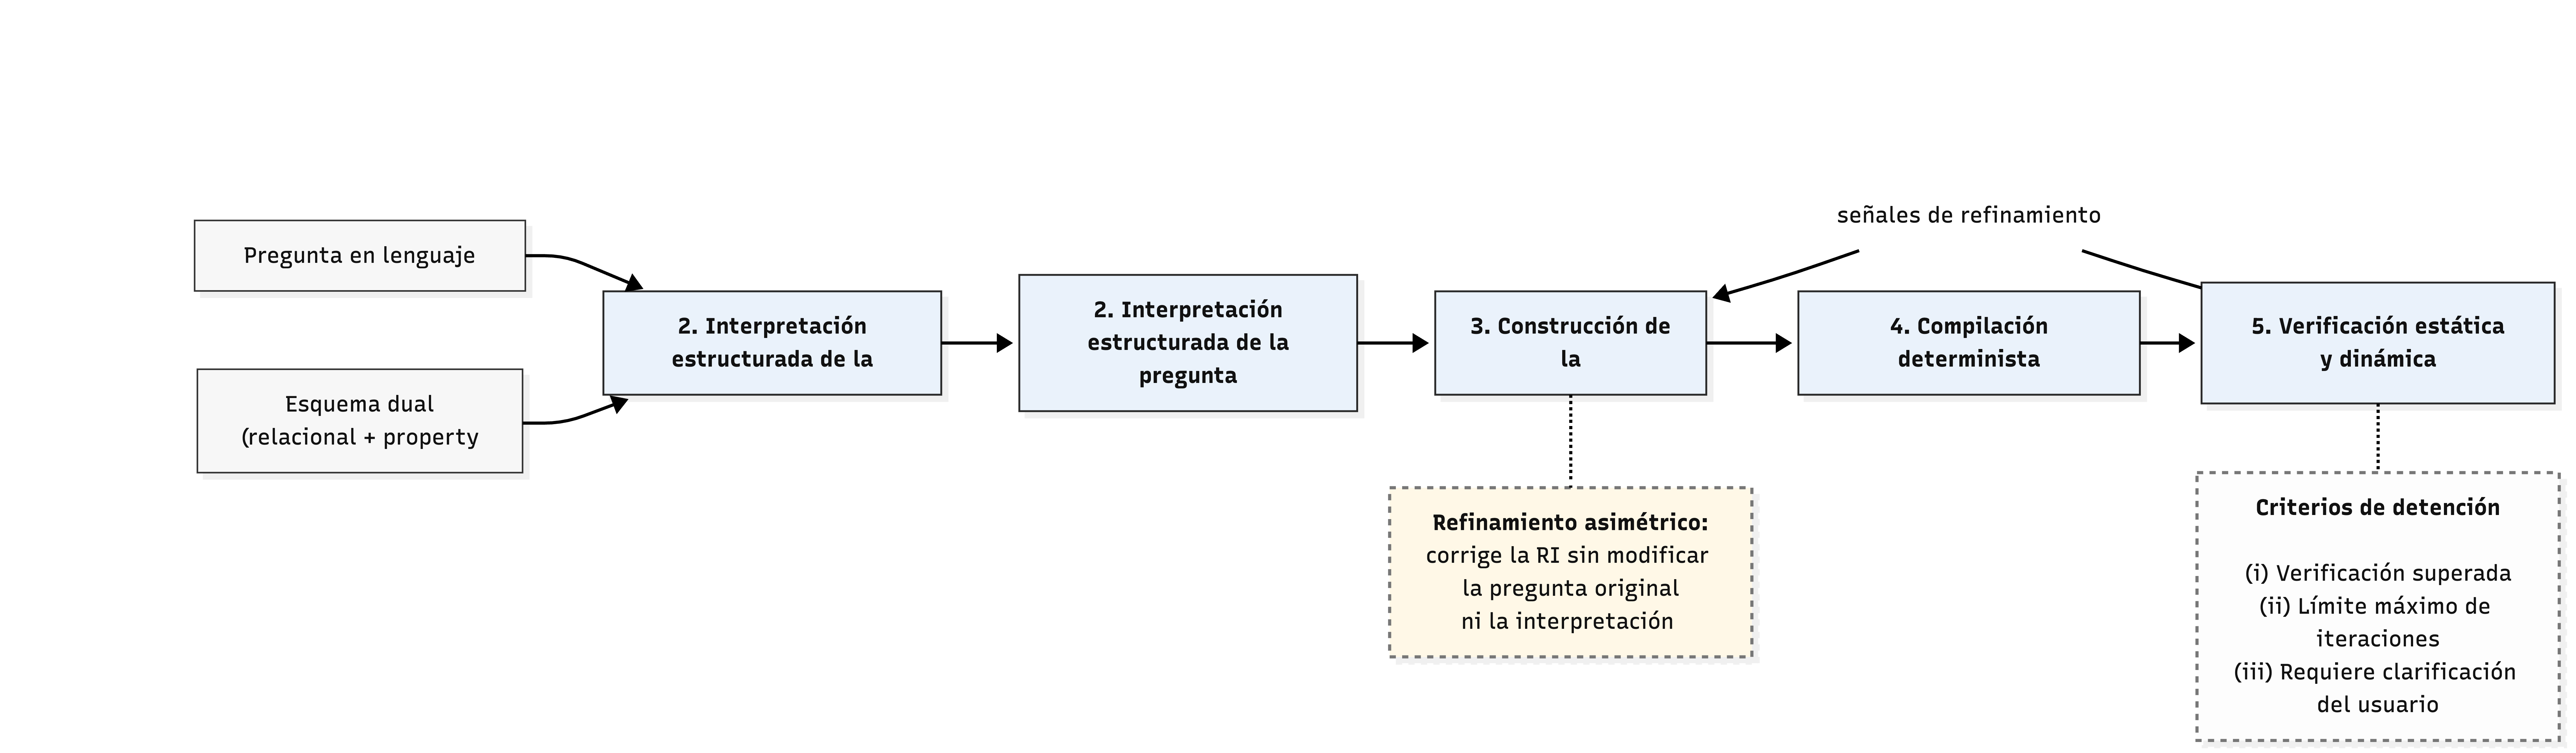
\includegraphics[width=\linewidth]{figs/Chap4/pipeline-general.png}
    \caption{Flujo metodológico general del \emph{pipeline} propuesto. Las
    cinco etapas secuenciales procesan la pregunta en lenguaje natural y el
    esquema dual (relacional y grafo de propiedad) hasta producir una
    consulta \ac{SQL}/\ac{PGQ} verificada.}
    \label{fig:pipeline-general}
\end{figure}

\begin{enumerate}
    \item \textbf{Pre-procesamiento y anclaje al esquema dual.} Esta etapa
    recibe como entrada la pregunta en lenguaje natural, el esquema
    relacional y la definición del grafo de propiedad. Su salida es un
    esquema proyectado, es decir, un subconjunto del esquema dual enriquecido
    con señales de relevancia, tales como tablas y columnas candidatas,
    vértices y aristas potencialmente implicados, así como \emph{cell-values}
    relevantes. Esta fase materializa el principio P1 y se apoya en ideas de
    anclaje al esquema y reducción del espacio de búsqueda reportadas en
    \cite{RSL-SQL2024, CHESS2024}.

    \item \textbf{Interpretación estructurada de la pregunta.} A partir de la
    pregunta y del esquema proyectado, esta etapa produce una descomposición
    explícita de la intención del usuario en componentes interpretables:
    entidades mencionadas, restricciones, proyecciones esperadas y tipo de
    razonamiento requerido. En particular, identifica si la consulta demanda
    razonamiento relacional, razonamiento sobre grafos o una combinación de
    ambos. Esta etapa se inspira en el paradigma de descomposición presentado
    en \cite{DIN-SQL2023, MAC-SQL2023}, extendiéndolo al contexto híbrido
    \ac{SQL}/\ac{PGQ}.

    \item \textbf{Construcción de la representación intermedia tipada.} Con
    base en la interpretación estructurada, se construye una instancia de la
    \ac{RI} propuesta. Esta etapa constituye el núcleo conceptual de la
    arquitectura, pues traduce la intención del usuario a una forma
    estructurada, tipada y validable antes de cualquier compilación al
    lenguaje de consulta final.

    \item \textbf{Compilación determinista a \ac{SQL}/\ac{PGQ}.} Una vez que
    la \ac{RI} satisface sus restricciones estructurales, se compila a una
    consulta concreta mediante reglas deterministas, sin intervención
    adicional del \ac{LLM}. De este modo, la generación estadística queda
    separada de la síntesis sintáctica final, y la consulta producida se
    ajusta por construcción a la gramática del estándar objetivo.

    \item \textbf{Verificación estática y dinámica.} La consulta compilada se
    somete, en primer lugar, a una verificación estática orientada a comprobar
    su consistencia estructural respecto del esquema dual. Si supera esta
    fase, se procede a una verificación dinámica mediante ejecución controlada
    sobre DuckPGQ~\cite{DuckPGQ}. Los errores detectados en cualquiera de
    estos dos niveles se transforman en señales de refinamiento que
    retroalimentan la etapa de construcción de la \ac{RI}.
\end{enumerate}

El bucle de refinamiento es asimétrico en el sentido que la
retroalimentación no modifica la pregunta original ni reabre la interpretación
de alto nivel de la etapa dos, sino que actúa exclusivamente sobre la
construcción de la \ac{RI}. Esta decisión responde al principio P2, ya que
concentra la corrección en el espacio donde la estructura puede manipularse de
forma explícita y verificable mediante reglas. El refinamiento concluye cuando
se satisface alguno de los siguientes criterios: (i) la verificación es
superada, (ii) se alcanza un número máximo de iteraciones, o (iii) el sistema
determina que la pregunta presenta una ambigüedad intrínseca que requiere
clarificación del usuario, en consonancia con lo planteado por
\cite{AmbiSQL}.






\section{Arquitectura y componentes}
\label{sec:prop-arquitectura}

\section{Implementación sobre la base experimental}
\label{sec:prop-implementacion}

\section{Justificación de decisiones de diseño}
\label{sec:prop-justificacion}

\section{Síntesis y transición}
\label{sec:prop-sintesis}
